\documentclass[10pt]{beamer}
\usepackage[english]{babel}
\usepackage{graphicx}
\usepackage{pgfkeys}
\usepackage{tikz}
\usepackage{amstext}
\usetheme{default}
\title[The SDHCAL technological proposal]{The SDHCAL technological prototype \\ Construction, first results and ongoing R\&D}
\author{L. Mirabito}
\institute{IPN Lyon, UCB Lyon, IN2P3, CNRS}
\date{November 11, 2014}

\begin{document}
% \AtBeginSection[]
% {
%   \begin{frame}<beamer>
%     \frametitle{Plan}
%     \tableofcontents[currentsection,currentsubsection]
%   \end{frame}
% }

\setbeamerfont{frametitle}{size=\huge,series=\bfseries}

\begin{frame}
  \titlepage
\end{frame}

\section{Introduction}
\begin{frame}[shrink=5]{Introduction}


  \begin{columns}
    \begin{column}{0.6\textwidth}
      \begin{block}{\small Context}
   	{\small The SDHCAL-GRPC is one of the two HCAL options proposed
          in the ILD Letter Of Intent (LOI). Modules are  made of 
          48 RPC chambers (6$\lambda_I$) equipped with 
          power-pulsed electronics readout.}   
      \end{block}
      
      \begin{block}{ \small SDHCAL-ILD}
        {\small The structure proposed for the SDHCAL-ILD :
          \par $ ~ \rightarrow$ Is self-supporting 
          \par $ ~\rightarrow$ Has negligible dead zones 
          \par $ ~ \rightarrow$ Eliminates projective cracks 
          \par $ ~ \rightarrow$ Minimizes barrel / endcap separation 
        }
      \end{block}

      \begin{block}{\small  Chamber challenges}
        {\small 
          \par $ ~ \rightarrow$ Thickness of only few mms
          \par $ ~ \rightarrow$ Homogeneity for large surfaces
          \par $ ~ \rightarrow$ Services from one side
          \par $ ~ \rightarrow$ Embedded power-pulsed electronics
          \par $ ~ \rightarrow$ Self-supporting mechanical structure 
          
        }
      \end{block}

    \end{column}

    \begin{column}{0.4\textwidth}
      \centerline{\includegraphics[height=0.45\textheight]{jpg/IldDhcal}}
      \centerline{\includegraphics[height=0.25\textheight]{jpg/m3Proto.jpg}}
      \centerline{\includegraphics[height=0.25\textheight]{jpg/DHCALProtoSchema}}
    \end{column}
  \end{columns}
\end{frame}

\begin{frame}{Detector Choice}

  \begin{block}{Glass Resistive Plate Chamber}
    \begin{columns}
      \begin{column}{0.5\textwidth}
        {
   	  \par $ ~ \rightarrow$ Thin, homogeneous, cost-effective
          \par $ ~ \rightarrow$ Avalanche $\simeq 1 mm$ radius: High granularity achievable
        }   
      \end{column}
      \begin{column}{0.5\textwidth}
        \centerline{\includegraphics[width=0.9\textwidth]{jpg/ShowerExample}}
      \end{column}
    \end{columns}
  \end{block}
  
  \pause   

  \begin{block}{  Semi Digital}
    \begin{columns}
      \begin{column}{0.5\textwidth}
        {
          \par $ ~ \rightarrow$ Saturation on 1 $cm^2$ pad in the core of hadronic showers 
          \par $ ~\rightarrow$ 2-bits semi-digital readout improves resolution
        }
      \end{column}

      \begin{column}{0.5\textwidth}
        \centerline{\includegraphics[width=0.9\textwidth]{jpg/DigitalSemiDigital}}
      \end{column}
    \end{columns}

  \end{block} 

\end{frame}
\section{Glass RPC }
\begin{frame}{GRPC design}

  \centerline{\includegraphics[width=0.9\textwidth,height=0.4\textheight]{jpg/GRPCSchema}}
  \pause   

  \begin{columns}
    \begin{column}{0.45\textwidth}
      \centerline{\includegraphics[width=0.9\textwidth]{jpg/GasFlow}}
    \end{column}
    \pause
    \begin{column}{0.45\textwidth}

      \centerline{\includegraphics[width=0.9\textwidth]{jpg/CoatingStudies}}
    \end{column}
  \end{columns}
  

\end{frame}
\begin{frame}[shrink=3]{Readout Electronic}
  \begin{block}{HardRoc ASIC}
    \begin{columns}
      \begin{column}{0.5\textwidth}
        {\small 
          developped by Omega
          \par $ ~ \rightarrow$ 64 channels, triggerless mode, 127 memory slots
          \par $ ~\rightarrow$  3 thresholds , range [10 fC,  15 pC]
          \par $ ~\rightarrow$  Channel gain : Uniformity correction
          \par $ ~\rightarrow$  Analog power switch: Power-pulsed capability, low consumption

        }
      \end{column}

      \begin{column}{0.5\textwidth}
        \centerline{\includegraphics[width=0.9\textwidth]{jpg/HR2Chip}}
        \centerline{\includegraphics[width=0.9\textwidth]{jpg/HR2GainAdjustement}}
      \end{column}

    \end{columns}
  \end{block}
  \pause
  \begin{block}{ASU PCB development}
    \begin{columns}
      \begin{column}{0.5\textwidth}
        {\small 
          \par $ ~ \rightarrow$ 8-Layers, buried vias, 50 x 33 cms
          \par $ ~\rightarrow$  Two 24 asics PCB connected with flat connectors
          \par $ ~\rightarrow$  DAQ board (DIF) controls and read the 48 daisy chained chips (developped by LAPP)
        }
      \end{column}

      \begin{column}{0.5\textwidth}
        \centerline{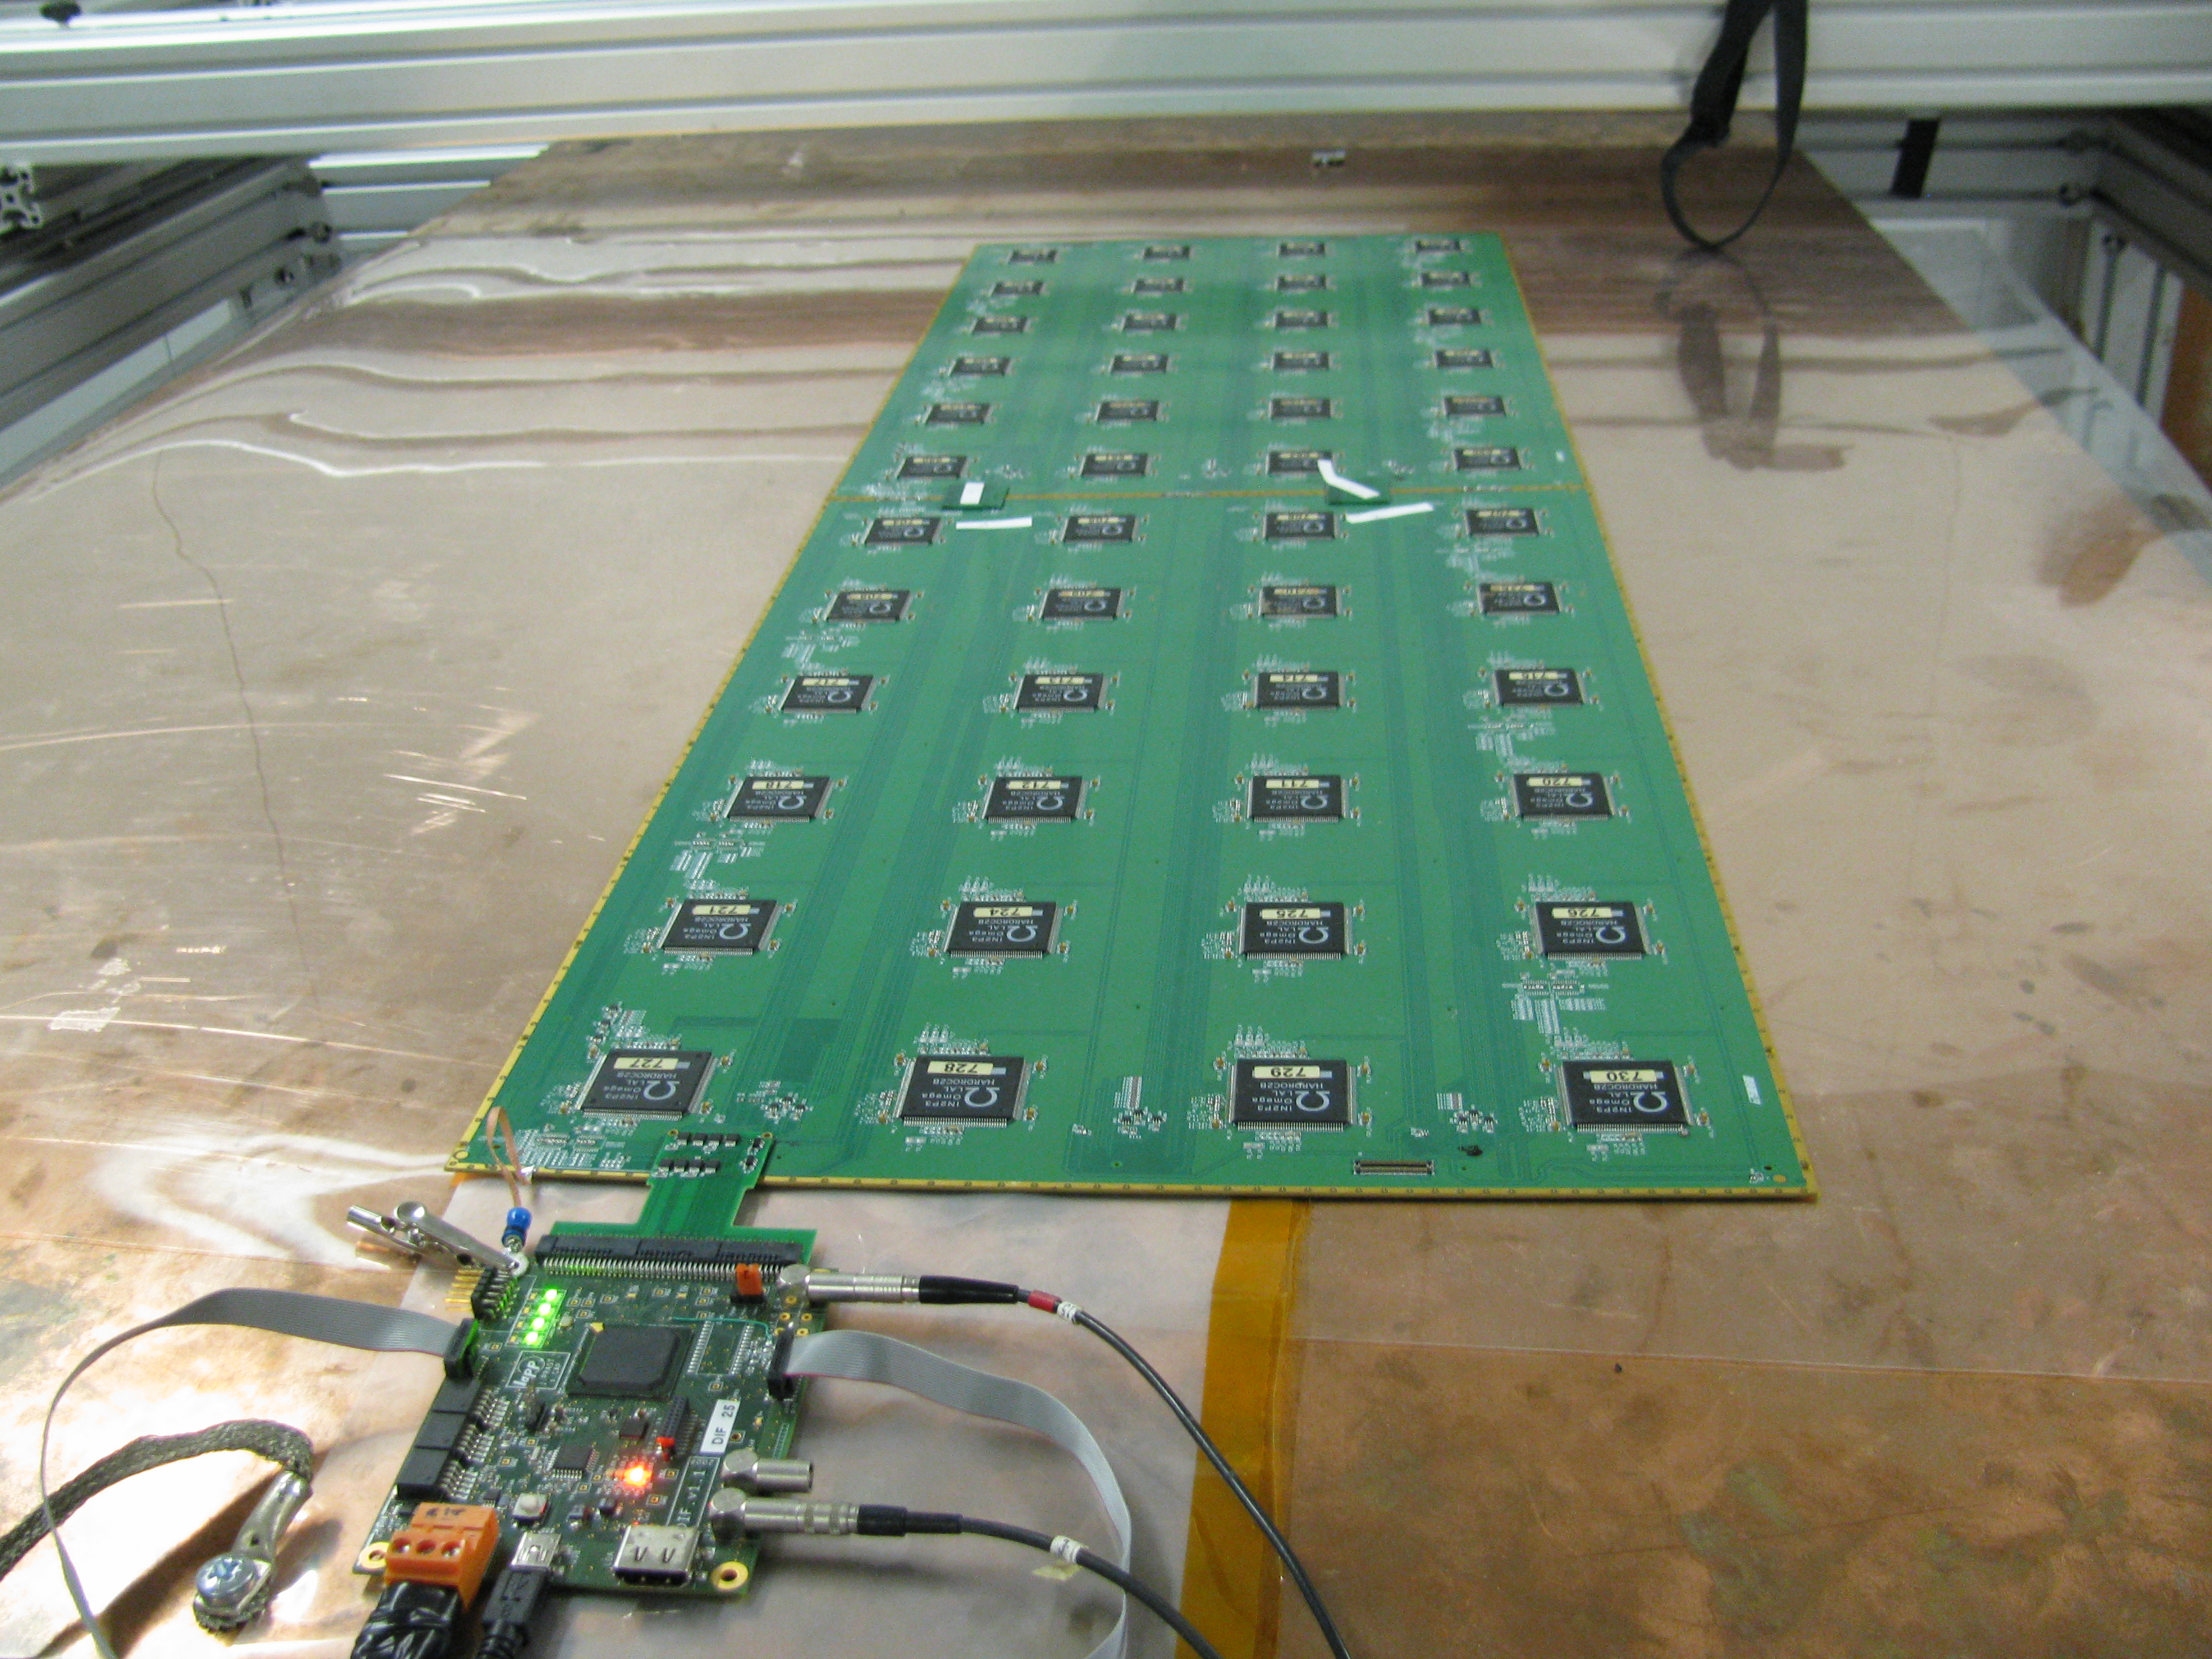
\includegraphics[width=0.9\textwidth]{jpg/DIFAsu}}
      \end{column}

    \end{columns}
  \end{block}
\end{frame}
\begin{frame}{Cassette assembly}
  \begin{columns}
    \begin{column}{0.5\textwidth}

      \centerline{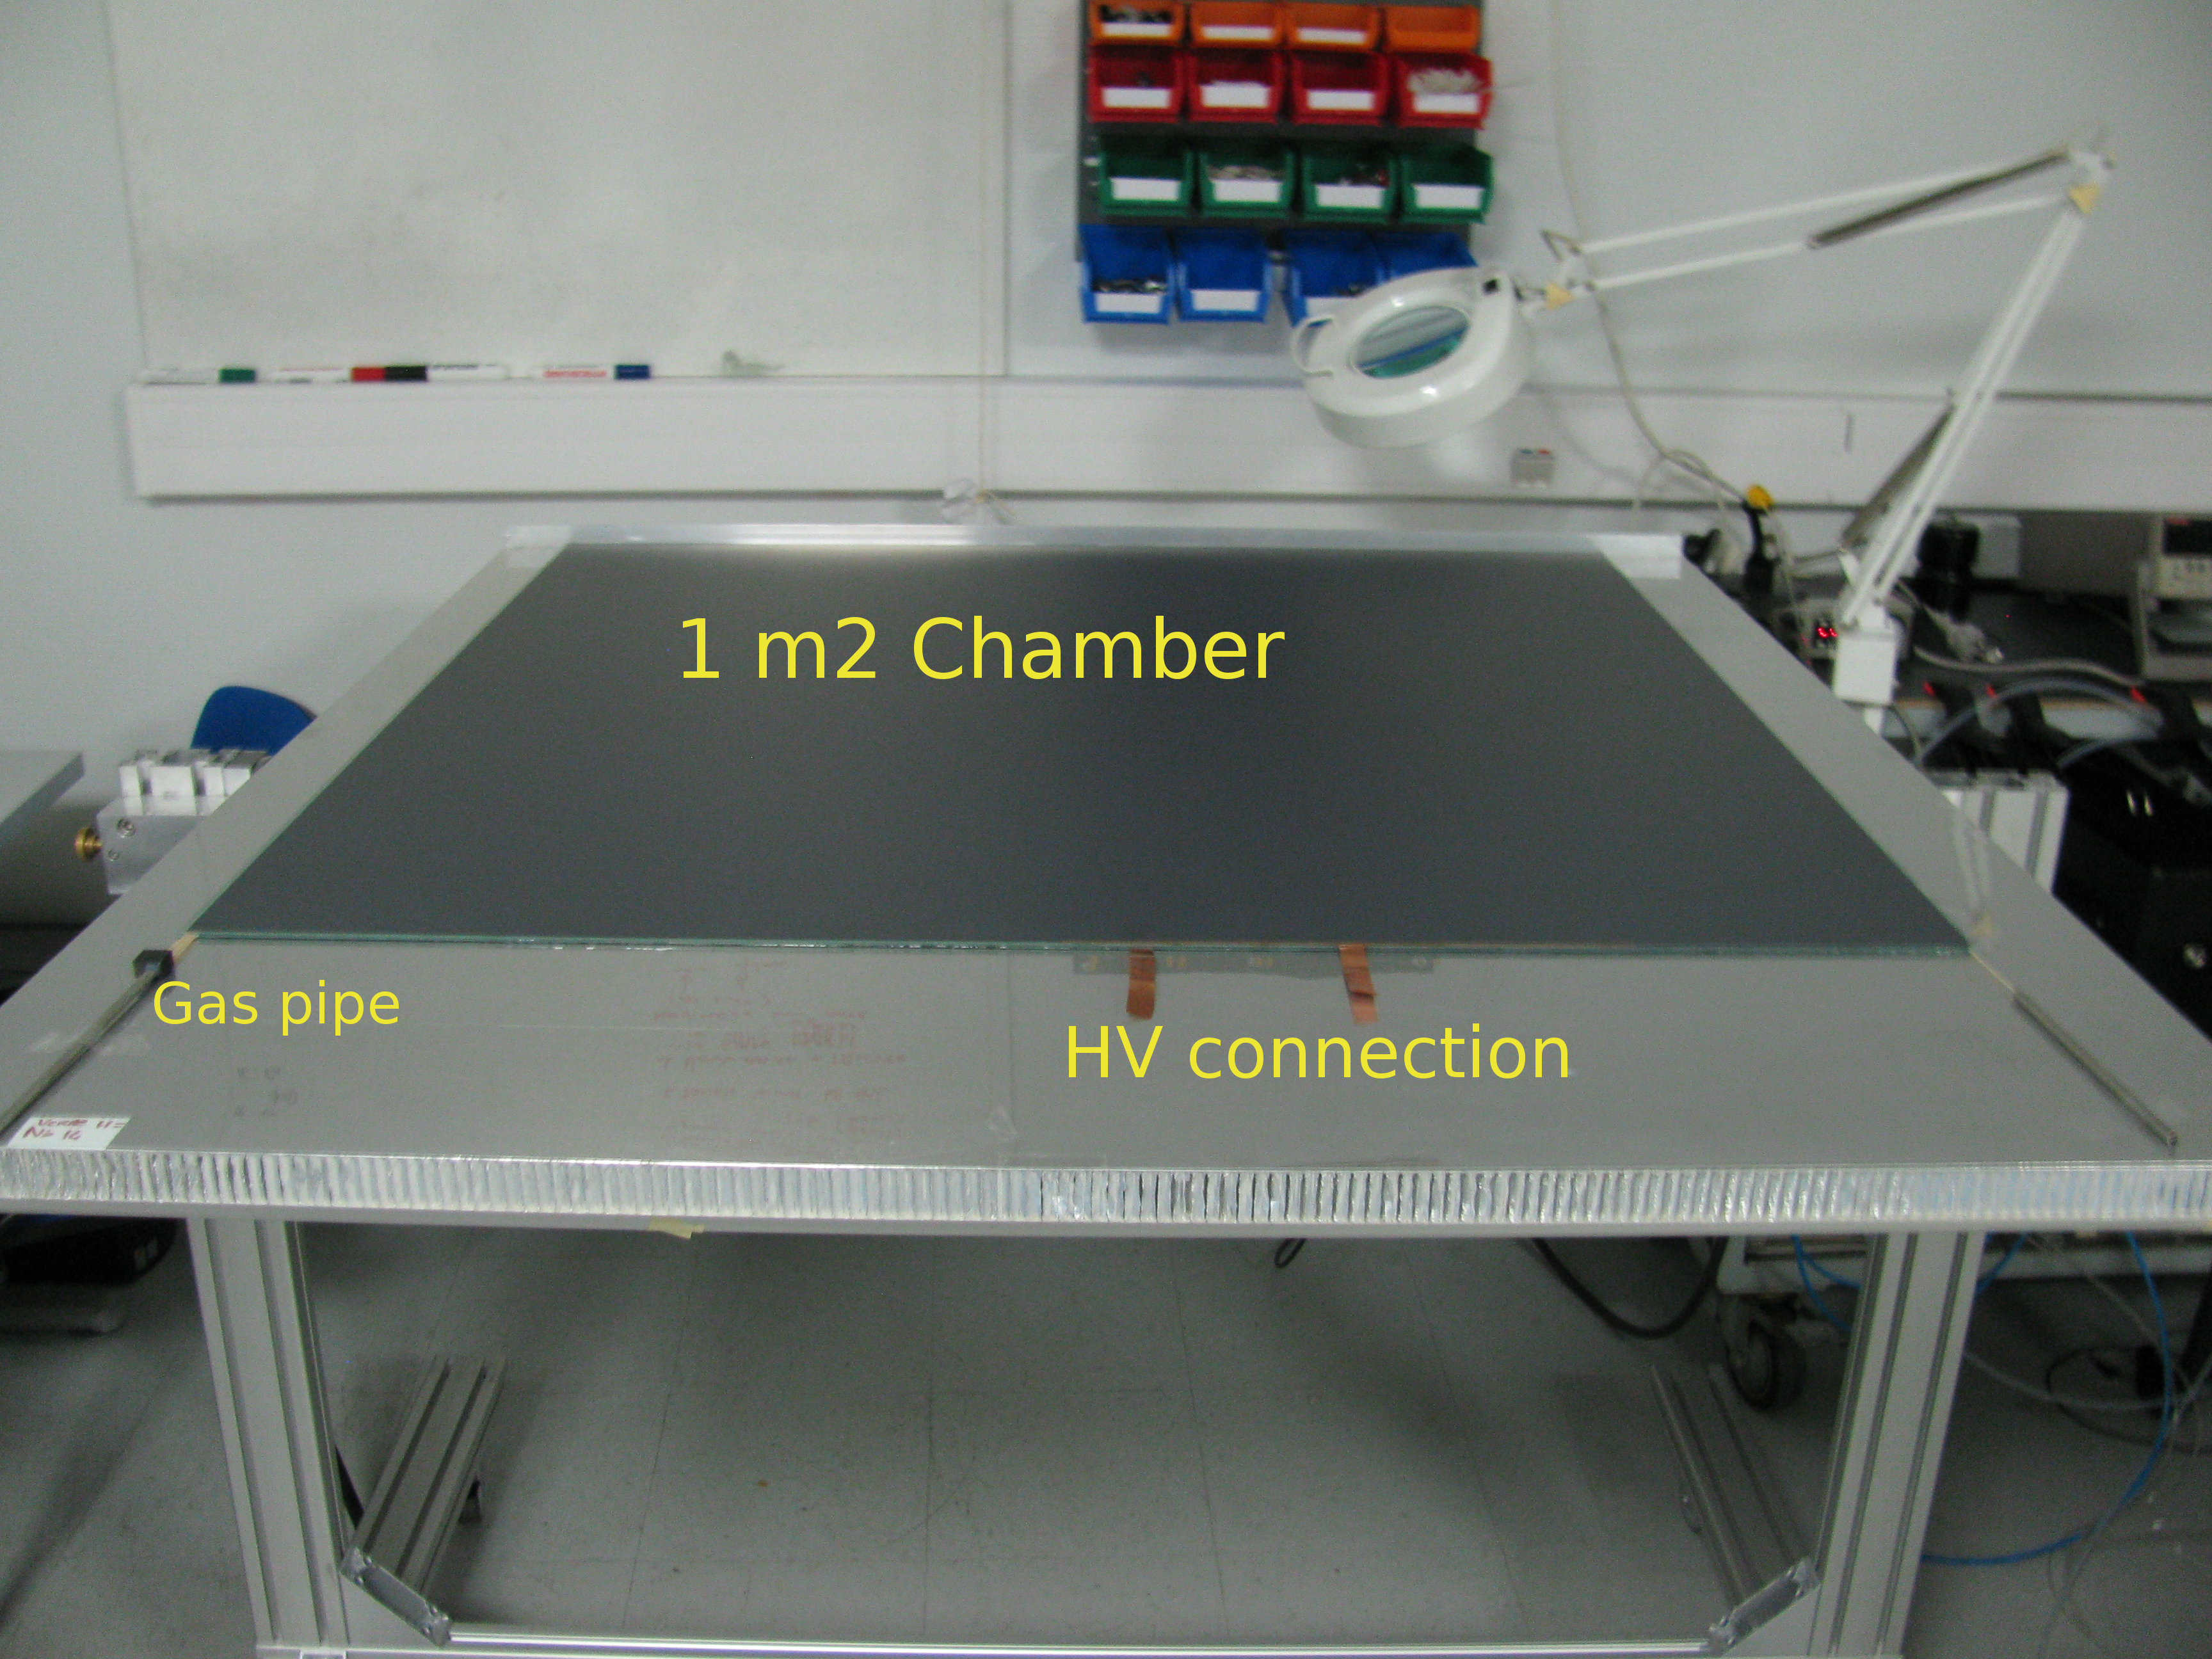
\includegraphics[width=0.9\textwidth]{jpg/ConstructionRPC}}
    \end{column}
    \pause
    \begin{column}{0.5\textwidth}


      \centerline{\includegraphics[width=0.9\textwidth]{jpg/1m2HR2}}
    \end{column}
  \end{columns}
  \begin{columns}
    \pause

    \begin{column}{0.5\textwidth}

      \centerline{\includegraphics[width=0.9\textwidth]{jpg/1m2Cover}}
    \end{column}
    \pause
    \begin{column}{0.5\textwidth}

      
      \centerline{\includegraphics[width=0.9\textwidth]{jpg/1m2Cassette}}
    \end{column}
  \end{columns}

\end{frame}

\begin{frame}{Acquisition system}
  \centerline{\includegraphics[width=0.9\textwidth,height=0.45\textheight]{jpg/DAQLinks}}
  \begin{block}{}
    \begin{itemize}

     \item Oracle configuration data base
     \item  Event building with CMS Event Event builder (XDAQ)
     \item  Up to 150 USB links on 4 PCs
     \item  Rate limited by USB1 links and  5 MHz readout of ASIC daisy chained 

    \end{itemize}
  \end{block}
\end{frame}
\begin{frame}{Chamber performances  }
  \begin{block}{Working point}
    \begin{itemize}
      \item Gas: TFE(92 \%), CO2 (5 \%), SF6 (2 \%)
      \item HV : -7.0 kV ( 20$^o$ C, 1020 mbar) 
      \item Efficiency $\simeq$ 95 \%
      \item Pad Multiplicity $\simeq$ 1.7
    \end{itemize}
  \end{block}
  \begin{block}{ Cosmic muons studies}
    \begin{columns}

      \begin{column}{0.5\textwidth}
        \centerline{\includegraphics[width=0.9\textwidth]{jpg/LocalEfficiency}}
      \end{column}
      \begin{column}{0.5\textwidth}
        \centerline{\includegraphics[width=0.9\textwidth]{jpg/LocalMultiplicity}}
      \end{column}
    \end{columns}
  \end{block}

\end{frame}
\begin{frame}{Chamber performances  }
  \begin{block}{Power-pulsed performances in 3T B field (H2-CERN)}
    \begin{columns}

      \begin{column}{0.5\textwidth}
        \centerline{\includegraphics[width=0.9\textwidth]{jpg/PowerPulsingPhoto}}
      \end{column}
      
      \begin{column}{0.5\textwidth}
        \centerline{\includegraphics[width=0.9\textwidth]{jpg/PowerPulsingHvScan}}
        %        \centerline{\includegraphics[width=0.9\textwidth]{jpg/CoatingStudies}}
      \end{column}
    \end{columns}
  \end{block}

\end{frame}
\section{ Technological prototype}
\begin{frame}[shrink=3]{Prototype construction}
  \begin{block}{}

    \begin{columns}

      \begin{column}{0.5\textwidth}
        \begin{block}{}
        { 
          Production and test of 
          \par $ ~\rightarrow$ 10500 HR2 chips  (LAL Omega)
          \par $ ~\rightarrow$  150 ASU + 300 interconnection PCBs
          \par $ ~ \rightarrow$ 170 DIF (LAPP) and 20 DCC (LLR)
        }
        \end{block}
      \end{column}
      
      \begin{column}{0.5\textwidth}
        \centerline{\includegraphics[width=0.9\textwidth]{jpg/ConstructionGantry.jpg}}
      \end{column}
    \end{columns}
  \end{block}
\begin{block}

    \begin{columns}

      \begin{column}{0.5\textwidth}
        \begin{block}{}
        {
          Production and test of 
          \par $ ~\rightarrow$ 50 chambers and cassettes
          \par $ ~\rightarrow$ 8 storage racks used as cosmic muon stand 
        }
        \end{block}
      \end{column}
      
      \begin{column}{0.5\textwidth}
        \centerline{\includegraphics[width=0.9\textwidth]{jpg/ConstructionRack.jpg}}
      \end{column}
    \end{columns}
  \end{block}

\end{frame}
\begin{frame}{Final integration at CERN}
\begin{columns}
 \begin{column}{0.5\textwidth}
\begin{block}{}
  \begin{itemize}
  \item Mechanical structure developped by CIEMAT
  \item HV and cooling services developped by Gent and Louvain
  \item Full assembly made at CERN before the beam tests     
  \end{itemize}
\end{block}
      \end{column}
      
      \begin{column}{0.5\textwidth}
 
        \centerline{\includegraphics[width=0.9\textwidth,height=0.5\textheight]{jpg/ConstructionStructure.jpg}}
        \centerline{\includegraphics[width=0.9\textwidth]{jpg/ConstructionInsertion.jpg}}

      \end{column}
    \end{columns}
\end{frame}

\begin{frame}{Beam tests in 2012}
  \begin{columns}
    \begin{column}{0.4\textwidth}
      \begin{block}{}
        \begin{itemize}
        \item 5 weeks of data taking on PS and SPS lines at CERN
        \item $\pi$ and e beams from 3 to 100 GeV allowing to study both hadronic and electromagnetic showers in a large energy range
         \item power pulsing mode (Analog on during spill) minimized the required cooling
         \item Trigger less mode $\rightarrow$ better daq efficiency, beam muons to monitor the rate and the chambers efficiency
        \end{itemize}
      \end{block}
    \end{column}
    \begin{column}{0.6\textwidth}
      \centerline{\includegraphics[width=0.9\textwidth,height=0.5\textheight]{jpg/1m3Photo.jpg}}
    \end{column}
  \end{columns}
\end{frame}

\begin{frame}{Showers}
  \begin{block}{10 Gev $\pi$ and e}
    \begin{columns}
      \begin{column}{0.5\textwidth}
        \centerline{\includegraphics[width=0.95\textwidth]{jpg/10GevPion.jpg}}
      \end{column}
      \begin{column}{0.5\textwidth}
        \centerline{\includegraphics[width=0.95\textwidth]{jpg/10GevElectron.jpg}}
      \end{column}
    \end{columns}
      
  \end{block}
  \begin{block}{50 Gev $\pi$ and e}
    \begin{columns}
      \begin{column}{0.5\textwidth}
        \centerline{\includegraphics[width=0.95\textwidth]{jpg/50GevPion.jpg}}
      \end{column}
      \begin{column}{0.5\textwidth}
        \centerline{\includegraphics[width=0.95\textwidth]{jpg/50GevElectron.jpg}}
      \end{column}
    \end{columns}

  \end{block}

\end{frame}

\begin{frame}{Commissioning}
\begin{block}{Noise Studies}
\begin{columns}
\begin{column}{0.3\textwidth}
  {\small
    \par $ ~ \rightarrow$  $ < 1 $ Hz/pad, $\simeq 0.35 $ Hit/ Bx (200 ns)
    \par $ ~ \rightarrow$ Locally high noise (mask or gain adjust)
  }  
\end{column}
\begin{column}{0.35\textwidth}
  \centerline{\includegraphics[width=0.95\textwidth]{jpg/hitsperclock.jpg}}
\end{column}
\begin{column}{0.35\textwidth}
  \centerline{\includegraphics[width=0.95\textwidth]{jpg/HitsMap.jpg}}
\end{column}
\end{columns}
\end{block}

\begin{block}{Threshold study}
\begin{columns}
\begin{column}{0.5\textwidth}
  {
    \par $ ~ \rightarrow$ Dedicated $\mu$ runs
    \par $ ~ \rightarrow$ Scan efficiency for the 3 thresholds
    \par $ ~ \rightarrow$ MC Polya response adjust from it
  }  
\end{column}
\begin{column}{0.5\textwidth}

  \centerline{\includegraphics[height=0.45\textheight]{jpg/thresholdscan.jpg}}

\end{column}
\end{columns}
\end{block}
\end{frame}
\begin{frame}{Analysis path}
\begin{block}{$\mu$ and e rejection}
\begin{columns}
\begin{column}{0.5\textwidth}
  {\small
    \par $ ~ \rightarrow $ Shower starts after 5th layer or more than 30 layers have at least 4 hits. (electron rejection)
    \par $ ~ \rightarrow $ Mean number of hits in fired layers above 2.2. ($\mu$ rejection)
    \par $ ~ \rightarrow $ At least 20 \% of the fired layers should have a spatial hit distribution with RMS $>$ 5cm (radiative $\mu$ rejection)
    \par $ ~ \rightarrow $ At least 4 hits in the first 5 layers (neutral rejection)   
  }  
\end{column}
\begin{column}{0.5\textwidth}

  \centerline{\includegraphics[height=0.45\textheight]{jpg/pionselection.jpg}}

\end{column}
\end{columns}

\end{block}
\pause
\begin{block}{Energy calibration}
\begin{columns}[t]
\begin{column}{0.5\textwidth}
{\small
 $ E_{R} =\alpha N_1 + \beta N_2 + \gamma N_3 $

where $ \alpha , \beta , \gamma $  are quadratic functions in $ N_{tot}=N_1+N_2+N_3 $ and  fitted from data
}
\end{column}
\begin{column}{0.5\textwidth}

  \centerline{\includegraphics[height=0.45\textheight]{jpg/evolution.jpg}}

\end{column}
\end{columns}
\end{block}
\end{frame}
\begin{frame}{Results}
\begin{columns}
\begin{column}{0.5\textwidth}

  \centerline{\includegraphics[height=0.9\textheight]{jpg/Energy-Linearity.jpg}}
\end{column}
\begin{column}{0.5\textwidth}

  \centerline{\includegraphics[width=1.15\textwidth]{jpg/Beam2012Resolution.jpg}}

\end{column}
\end{columns}
\end{frame}

\begin{frame}{Current software improvements}
\begin{columns}
\begin{column}{0.5\textwidth}
  {
    \par Tagging MIPs hits (Hough transform,combinatorial) separatly in $E_R$ fit, improves resolution from 7\%- 15 \%
  }

  \centerline{\includegraphics[width=0.9\textwidth]{jpg/Beam2012Hough.jpg}}
\end{column}
\begin{column}{0.5\textwidth}
  {
    \par New Shower reconstruction algorithm Arbor (MST based) improves shower separation
  }
  \centerline{\includegraphics[width=1.15\textwidth]{jpg/Beam2012Arbor.jpg}}
\end{column}
\end{columns}

\end{frame}

\section{Future}

\begin{frame}{Next data taking}
\begin{block}{Improve statistic}
\begin{itemize}
\item USB2 readout improves DAQ efficiency from 7 \% to 40 \%
\item Some 2012 runs were taken with $> 100$ Hz/pad, efficiency is currently corrected. Long low intensity runs needed 
\item Dedicated e runs to improve MC tuning 
\end{itemize}
\end{block}
\pause
\begin{block}{ New DAQ}
\begin{itemize}
\item Low consumption, integrated PC (raspberry pi), one for 4 chambers
\item Lighter DAQ framework (DIM)
\end{itemize}

\end{block}
\end{frame}

\begin{frame}{2 m long chambers}
\begin{block}{New gas distribution system}
  \centerline{\includegraphics[width=1.15\textwidth]{jpg/gasflow2m.jpg}}
\end{block}
\begin{block}{New mechanical structure}
  \centerline{\includegraphics[width=1.15\textwidth]{jpg/2mmechanic.jpg}}
\end{block}
\end{frame}
\begin{frame}[shrink=2]{ New electronic}
\begin{columns}
\begin{column}{0.5\textwidth}
\begin{block}{HardROC3 (Omega)}
\begin{itemize}
\item Independant 8-slots buffer per channel
\item I2C configuration
\item Better dynmamic range 
\end{itemize}

\end{block}
\centerline{\includegraphics[width=0.95\textwidth]{jpg/HR3.jpg}}

\end{column}
\begin{column}{0.5\textwidth}
\begin{block}{DIF3 (CIEMAT)}
\begin{itemize}
\item One DIF per plane (432 chips in 12 paralell lines)
\item Ethernet (commercial chip) readout, TTC clock \& commands
\item Spare SFP cage for bi-directionnal serial link implemnentation (GBT)
\end{itemize}

\end{block}
\centerline{\includegraphics[width=0.75\textwidth]{jpg/DIF3.jpg}}

\end{column}
\end{columns}
\end{frame}


\end{document}
